\documentclass[12pt]{article}
\usepackage{setspace, graphicx, fullpage, amssymb, amsmath, epsfig, natbib, array, multirow, hyperref}
\usepackage{amsfonts, bm} 
\usepackage{dcolumn}
\usepackage{subfigure, float} 
\usepackage[margin=1in]{geometry} 
\usepackage{verbatim}
\usepackage{url}
\usepackage{enumerate}
\usepackage{morefloats}
\usepackage{caption}
\newcolumntype{d}[1]{D{.}{.}{#1}} 

\newcommand\fnote[1]{\captionsetup{font=small}\caption*{#1}}

\begin{document}

\section{Overview}

At our previous meeting we decided to:

\begin{itemize}
	\item Consider alternative placebo tests to seniority
	
	\item Make additional improvements to prepare it for outside critique and reworking by William and Craig
\end{itemize}

\subsection{Alternative Placebo Tests}

If we are unhappy with the present use of higher seniority as a placebo test (given the fact that a higher seniority member will more often be nearer election or otherwise) we will need to select something else which would meaningfully separate same-state Senator pairs. Here I lay out a few additional possibilities:

The main alternative I can think of which would be related to reelection would be the number of votes cast in a particular Congress. A possible alternative mechanism would be that those up for reelection are not less responsive to the party because they are taking their constituents into greater account but instead because they are less present in Washington. Of course, this would also likely mean that they were spending more time in their state.

Resulting estimates below:

\begin{figure}[H]
	\centering
	\caption{Senate Rate of Voting With Party by Vote Type}
	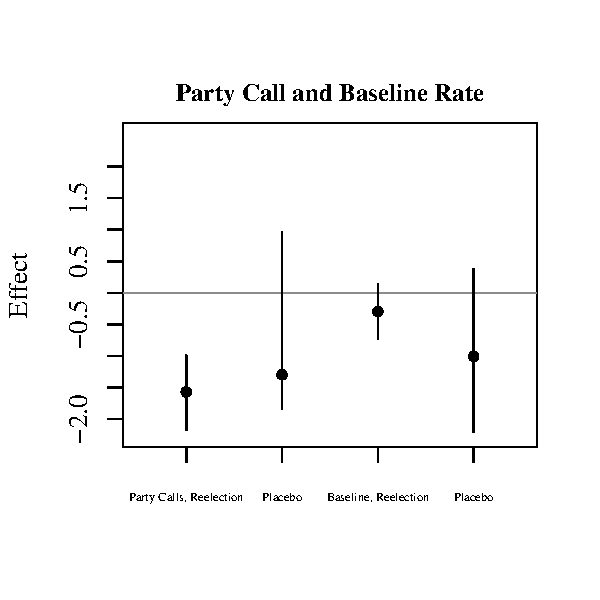
\includegraphics[width = 10cm]{C:/Users/Ethan/Documents/GitHub/partycalls/plots/senate-diff-in-diff-coeff-vote-placebo.pdf}
	
\end{figure}

As can be seen, this does not function well for showing the relationship, likely because these Senators are closer to their constituents. 

\clearpage

\doublespacing
	
\section{Paper, Draft 7}

\begin{center}
{\Large Who Heeds the Call in the U.S. Senate?}

{\large Reelection and Member Responsiveness to the Party}
\end{center}

\begin{abstract}
	\singlespacing
	\noindent
	In this paper, we replicate the findings of Minozzi \& Volden (2013) with some modifications of their methodology. We show that their hypotheses regarding party unity coming through the party working to unite more extreme (rather than more moderate) members holds not only in the House, but also the Senate. Further, we show the usefulness of separating votes in this way by considering changes in member behavior when they are up for reelection.
\end{abstract}



\subsection{Introduction}

Minozzi \& Volden (2013) developed the notion of the ``party call'' vote as one in which the party is clearly present alongside ideology. Party call votes were hypothesized by the authors to produce party unity, not through pressuring of moderates, but calling on members to support the position of the party. This hypothesis - the ``responsive extremists hypothesis'' - held that members on the tails would see the benefit of aiding the party brand and thus would more often get in line with these votes than would moderates.

This paper is written with the intention of replicating Minozzi \& Volden's work on party calls in the House, with extensions into later Congresses and the Senate. We view the party call as a valuable tool in explaining the behavior of members of Congress in relation to parties. We recognize that it is dangerous to attribute legislator behavior either to party or ideology given the high correlation between these characteristics (Krehbiel, 1993; Lee, 2009). Analyzing Congress with the use of party calls allows for the viewing of votes which party is a clear factor in addition to ideology. The Senate has typically been viewed as a less partisan chamber, but partisanship is presently on an upward trend within it (Theriault, 2013; Smith, 2014). For this reason, we expect to find party calls in the Senate, particularly in later Congresses, and for their influence to be similar to what Minozzi \& Volden found in the House of Representatives.

As an additional test, we consider an area of member behavior elsewhere shown to change member response to the party : proximity reelection in the Senate (Levitt, 1996). Members' primary goal is to be reelected (Mayhew, 1974). Legislators who are out of line with their district or who seem to be merely following the party will be electorally punished (Canes-Wrone, Brady \& Cogan, 2002; Carson et al., 2010). Party call votes could give members a clear opportunity to differentiate themselves from the party in the eyes of their constituents. Thus, we should expect Senators to behave more similarly to 

We find, as hypothesized, that party calls are present in the Senate. Further, we are able to show rigorously that it is on party call votes votes which we see changes to member behavior as reelection approaches. As expected, Senators are less likely to vote with the party on party call votes - but not other vote types - when they are up for reelection at the end of a Congress. We take this as strong evidence that the party call vote is explaining the place of the party in Congressional roll call behavior. In the next section we show the results of our replication with the section following it dedicated to additional tests concerning reelection before concluding the paper.

\subsection{Replication}

In this section we detail the results of our extended replication. This analysis involved the use of an algorithm which sorted votes into party calls and party free votes based on whether vote choice was significantly predicted by party status in addition to ideology. Member ideology is calculated on the party free votes from the previous iteration of the algorithm for each iteration. Our model is a modified version of the one described in Minozzi \& Volden (2013). Ideological extremism for our analyses is member party free ideal point from the final iteration, with sign reversed for Democrats (so that it is higher for members of each party as they become more extreme).\footnote{A more thorough overview of the methodology is detailed in an appendix.}

We find that party calls are in both the House and Senate. Additionally, we find that in both chambers their incidence has been on an upward trend during our period of analysis (1973 - 2013). We believe this trend merits further investigation, but initially take it as evidence of increased partisanship in recent decades, in line with others' findings (Lee, 2009, 2015; Theriault, 2013; Smith, 2014). This trend holds regardless of which party is in the majority in the chamber.


\begin{figure}[H]
	\centering
	\caption{Party Calls as a Percentage of Votes, Congresses 93-112}
	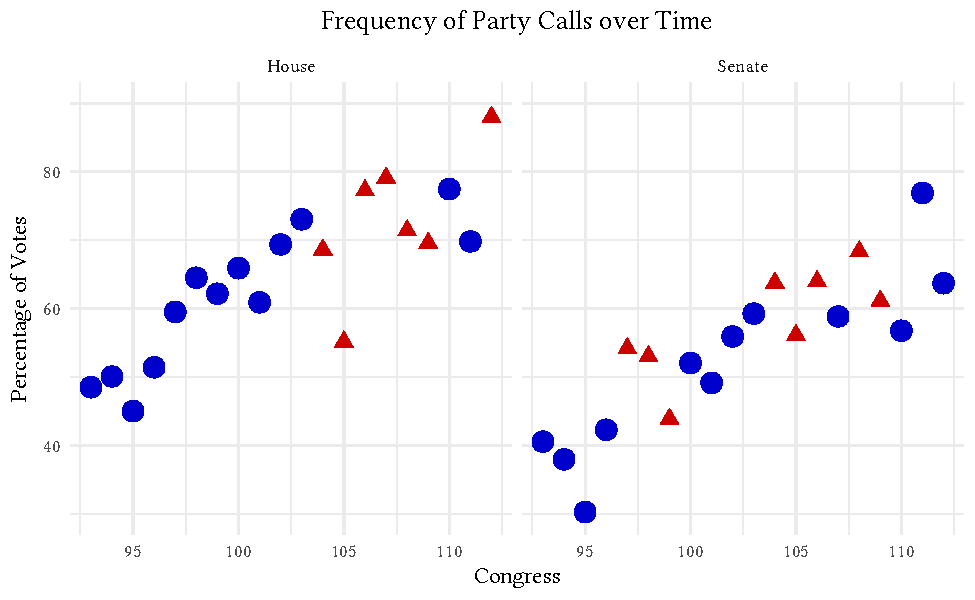
\includegraphics[width = \textwidth]{C:/Users/Ethan/Documents/GitHub/partycalls/plots/party_call_percent_both.pdf}
	\fnote{\textit{Note}: This figure shows the percentage of votes classified as party calls per Congress in each chamber. Blue circles denote Democrat majority Congresses while Red triangles denote Republican majority Congresses.}
\end{figure}

Models based on those of Minozzi \& Volden show the responsive extremists hypothesis to hold. In both chambers we find that increased ideological extremism leads to increased responsiveness on party call votes. This finding holds whether we consider all members together, or divide them by party or majority status.

%We find that Southern Democrats are less responsive to the party than are other Democrats, unsurprising since they have typically been near the chamber median. We also note that the power committee variable we constructed for the Senate (based on membership in a top 4 committee) carries little predictive power, either in terms of substantive power or statistical significance. This is not entirely unexpected, since this is a variable we included less because we believed it had meaning to Senators and more for model comparability. We also note that in both chambers increased same party presidential vote share within one's constituency makes Democrats more likely to respond to a party call but reduces the chances of a Republican doing so.

\begin{table}[H]
	\begin{center}
		\singlespacing
		\small
		\caption{House Responsiveness to Party Calls}
		%\footnotesize
		\begin{tabular}{l c c c c c }
			\hline
			& All & Democrats & Republicans & Majority & Minority \\
			\hline
			Ideological Extremism & $7.766^{***}$  & $8.350^{***}$  & $5.873^{***}$  & $6.713^{***}$  & $8.655^{***}$  \\
			& $(0.130)$      & $(0.168)$      & $(0.207)$      & $(0.157)$      & $(0.201)$      \\
			Baseline Rate of Voting With Party              & $0.575^{***}$  & $0.636^{***}$  & $0.414^{***}$  & $0.522^{***}$  & $0.632^{***}$  \\
			& $(0.012)$      & $(0.015)$      & $(0.020)$      & $(0.015)$      & $(0.020)$      \\
			Vote Share            & $-0.007$       & $-0.058^{***}$ & $0.021$        & $-0.125^{***}$ & $-0.109^{***}$ \\
			& $(0.012)$      & $(0.013)$      & $(0.022)$      & $(0.015)$      & $(0.019)$      \\
			Pres. Vote Share      & $0.028^{**}$   & $0.099^{***}$  & $-0.098^{***}$ & $0.204^{***}$  & $0.185^{***}$  \\
			& $(0.010)$      & $(0.011)$      & $(0.020)$      & $(0.012)$      & $(0.018)$      \\
			Party Leader                 & $1.811^{***}$  & $1.972^{**}$   & $2.787^{***}$  & $2.627^{***}$  & $1.843^{**}$   \\
			& $(0.497)$      & $(0.599)$      & $(0.761)$      & $(0.647)$      & $(0.653)$      \\
			Committee Chair                  & $4.960^{***}$  & $2.552^{***}$  & $9.779^{***}$  & $1.964^{***}$  &                \\
			& $(0.456)$      & $(0.498)$      & $(0.803)$      & $(0.444)$      &                \\
			Power Committee                  & $2.756^{***}$  & $1.801^{***}$  & $2.931^{***}$  & $2.972^{***}$  & $1.135^{**}$   \\
			& $(0.235)$      & $(0.275)$      & $(0.374)$      & $(0.269)$      & $(0.361)$      \\
			Best Committee          & $-0.169^{***}$ & $-0.038^{*}$   & $-0.240^{***}$ & $-0.178^{***}$ & $-0.161^{***}$ \\
			& $(0.016)$      & $(0.019)$      & $(0.025)$      & $(0.019)$      & $(0.023)$      \\
			Female                 & $1.173^{***}$  & $0.615$        & $-0.078$       & $0.037$        & $2.228^{***}$  \\
			& $(0.322)$      & $(0.353)$      & $(0.574)$      & $(0.404)$      & $(0.442)$      \\
			African American                   & $1.835^{***}$  & $-0.470$       & $5.089$        & $-3.014^{***}$ & $3.402^{***}$  \\
			& $(0.429)$      & $(0.441)$      & $(2.972)$      & $(0.536)$      & $(0.610)$      \\
			Latino                 & $3.221^{***}$  & $1.711^{***}$  & $2.405^{*}$    & $2.453^{***}$  & $3.191^{***}$  \\
			& $(0.507)$      & $(0.514)$      & $(1.153)$      & $(0.626)$      & $(0.705)$      \\
			South                  & $-0.922^{***}$ & $-2.640^{***}$ & $3.610^{***}$  & $-2.180^{***}$ & $-0.667^{*}$   \\
			& $(0.205)$      & $(0.276)$      & $(0.329)$      & $(0.244)$      & $(0.313)$      \\
			Seniority              & $-0.053$       & $0.049$        & $-0.334^{***}$ & $0.011$        & $0.015$        \\
			& $(0.028)$      & $(0.031)$      & $(0.050)$      & $(0.034)$      & $(0.041)$      \\
			Freshman               & $0.834^{**}$   & $-0.058$       & $1.167^{*}$    & $0.346$        & $-0.456$       \\
			& $(0.297)$      & $(0.356)$      & $(0.464)$      & $(0.348)$      & $(0.446)$      \\
			Intercept            & $30.952^{***}$ & $21.282^{***}$ & $53.412^{***}$ & $30.032^{***}$ & $12.343^{***}$ \\
			& $(1.217)$      & $(1.495)$      & $(2.174)$      & $(1.390)$      & $(2.106)$      \\
			\hline
			\multicolumn{6}{l}{\scriptsize{$^{***}p<0.001$, $^{**}p<0.01$, $^*p<0.05$}}
		\end{tabular}
	\fnote{Results are produced by OLS regressions for all members for the entire period in the first column, with additional analyses for all Democrats and Republicans as well as all members of the Majority and Minority party in Congresses 93-112 in the House of Representatives. Most variables provided by the Legislative Effectiveness Project, committee data come from Charles Stewart's data page, and vote share data provided by Gary Jacobson.}
	\end{center}
\end{table}

\begin{table}[H]
	\begin{center}
		\singlespacing
		\small
		\caption{Senate Responsiveness to Party Calls}
		%\footnotesize
		\begin{tabular}{l c c c c c }
			\hline
			& All & Democrats & Republicans & Majority & Minority \\
			\hline
			Ideological Extremism & $6.239^{***}$  & $3.136^{***}$ & $7.792^{***}$  & $4.708^{***}$  & $7.949^{***}$ \\
			& $(0.252)$      & $(0.409)$     & $(0.357)$      & $(0.315)$      & $(0.400)$     \\
			Baseline Rate of Voting with Party              & $0.737^{***}$  & $0.759^{***}$ & $0.742^{***}$  & $0.702^{***}$  & $0.702^{***}$ \\
			& $(0.021)$      & $(0.030)$     & $(0.031)$      & $(0.025)$      & $(0.035)$     \\
			Up For Reelection    & $-0.908^{*}$   & $-0.630$      & $-1.436^{**}$  & $-0.951^{*}$   & $-1.204^{*}$  \\
			& $(0.353)$      & $(0.426)$     & $(0.538)$      & $(0.411)$      & $(0.603)$     \\
			Retiree                & $2.103^{**}$   & $1.599$       & $2.290^{*}$    & $1.816^{*}$    & $2.575^{*}$   \\
			& $(0.693)$      & $(0.897)$     & $(0.997)$      & $(0.850)$      & $(1.110)$     \\
			Vote Share            & $0.029$        & $-0.053^{*}$  & $0.149^{***}$  & $-0.012$       & $0.076^{*}$   \\
			& $(0.018)$      & $(0.022)$     & $(0.028)$      & $(0.021)$      & $(0.030)$     \\
			Presidential Vote Share      & $0.097^{***}$  & $0.234^{***}$ & $-0.134^{***}$ & $0.182^{***}$  & $0.006$       \\
			& $(0.018)$      & $(0.024)$     & $(0.031)$      & $(0.020)$      & $(0.032)$     \\
			Party Leader                 & $1.604^{**}$   & $2.218^{**}$  & $0.910$        & $1.441^{*}$    & $1.940^{*}$   \\
			& $(0.539)$      & $(0.712)$     & $(0.776)$      & $(0.661)$      & $(0.899)$     \\
			Committee Chair                  & $2.105^{***}$  & $0.852$       & $3.626^{***}$  & $-0.017$       &               \\
			& $(0.452)$      & $(0.543)$     & $(0.700)$      & $(0.517)$      &               \\
			Power Committee       & $-0.684$       & $-0.855$      & $-0.325$       & $-0.052$       & $-1.468$      \\
			& $(0.620)$      & $(0.772)$     & $(0.924)$      & $(0.719)$      & $(1.064)$     \\
			Best Committee        & $0.163$        & $0.237$       & $0.008$        & $0.027$        & $0.373^{*}$   \\
			& $(0.101)$      & $(0.124)$     & $(0.154)$      & $(0.118)$      & $(0.174)$     \\
			Female                 & $2.041^{**}$   & $1.690^{*}$   & $0.451$        & $0.532$        & $4.256^{***}$ \\
			& $(0.638)$      & $(0.730)$     & $(1.132)$      & $(0.758)$      & $(1.113)$     \\
			African American                   & $-4.769$       & $-1.164$      & $-10.789^{*}$  & $1.531$        & $-5.519$      \\
			& $(2.486)$      & $(2.789)$     & $(4.278)$      & $(4.184)$      & $(3.219)$     \\
			Latino                 & $5.717^{**}$   & $1.814$       & $7.264^{**}$   & $4.781^{*}$    & $6.253$       \\
			& $(1.816)$      & $(2.198)$     & $(2.779)$      & $(1.878)$      & $(3.506)$     \\
			South                  & $0.613$        & $-1.690^{**}$ & $0.872$        & $0.054$        & $1.085$       \\
			& $(0.362)$      & $(0.557)$     & $(0.578)$      & $(0.427)$      & $(0.622)$     \\
			Seniority              & $0.002$        & $0.041$       & $-0.024$       & $0.077$        & $0.118$       \\
			& $(0.044)$      & $(0.052)$     & $(0.072)$      & $(0.060)$      & $(0.070)$     \\
			Freshman               & $0.859$        & $0.769$       & $0.358$        & $0.600$        & $0.996$       \\
			& $(0.566)$      & $(0.708)$     & $(0.842)$      & $(0.631)$      & $(1.032)$     \\
			Intercept            & $11.611^{***}$ & $9.447^{**}$  & $18.182^{***}$ & $16.365^{***}$ & $10.799^{**}$ \\
			& $(2.274)$      & $(2.906)$     & $(3.489)$      & $(2.644)$      & $(4.009)$     \\
			\hline
			R$^2$                  & 0.632          & 0.689         & 0.641          & 0.684          & 0.615         \\
			Adj. R$^2$             & 0.629          & 0.684         & 0.635          & 0.679          & 0.608         \\
			Num. obs.              & 1993           & 1042          & 951            & 1052           & 843           \\
			RMSE                   & 6.967          & 6.118         & 7.255          & 5.865          & 7.749         \\
			\hline
			\multicolumn{6}{l}{\scriptsize{$^{***}p<0.001$, $^{**}p<0.01$, $^*p<0.05$}}
		\end{tabular}
	\fnote{Results are produced by OLS regressions for all members for the entire period in the first column, with additional analyses for all Democrats and Republicans as well as all members of the Majority and Minority party in Congresses 93-112 in the Senate. Most variables provided by the Legislative Effectiveness Project, with supplementary data for committees from Charles Stewart's Congressional data and retirement data from the Congressional Bioguides.}
	\end{center}
\end{table}

In Table 2, we see strong evidence of member responsiveness to party calls declining as they approach reelection. Across all subgroups this coefficient is negative, and the effect viewed is significant for all members taken together as well as all subgroupings except Democrats. Before we move on to more specific considerations of reelection, however, we consider the relationship between ideological extremism and response to party calls for each Congress within each chamber of analysis.

\begin{figure}[H]
	\centering
	\caption{House Ideological Extremism Coefficient Plot}
	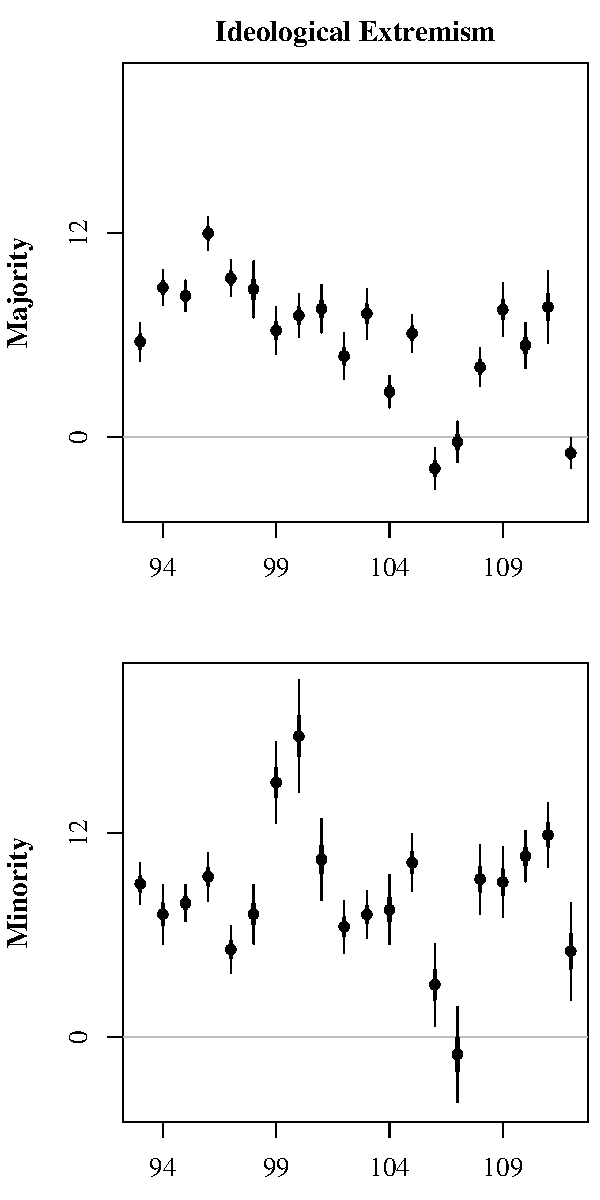
\includegraphics[width = 7cm]{C:/Users/Ethan/Documents/GitHub/partycalls/plots/who-heeds-figure2-replication_lm.pdf}
	\fnote{This coefficient plot is produced by the same formula shown in the House regression table with results decomposed by individual Congresses for the Majority and Minority parties. Coefficients shown are for the effect of ideological extremism on party free votes in relation to party call votes. 50\% and 95\% confidence intervals are shown from the points.}
\end{figure}

\begin{figure}[H]
	\centering
	\caption{Senate Ideological Extremism Coefficient Plot}
	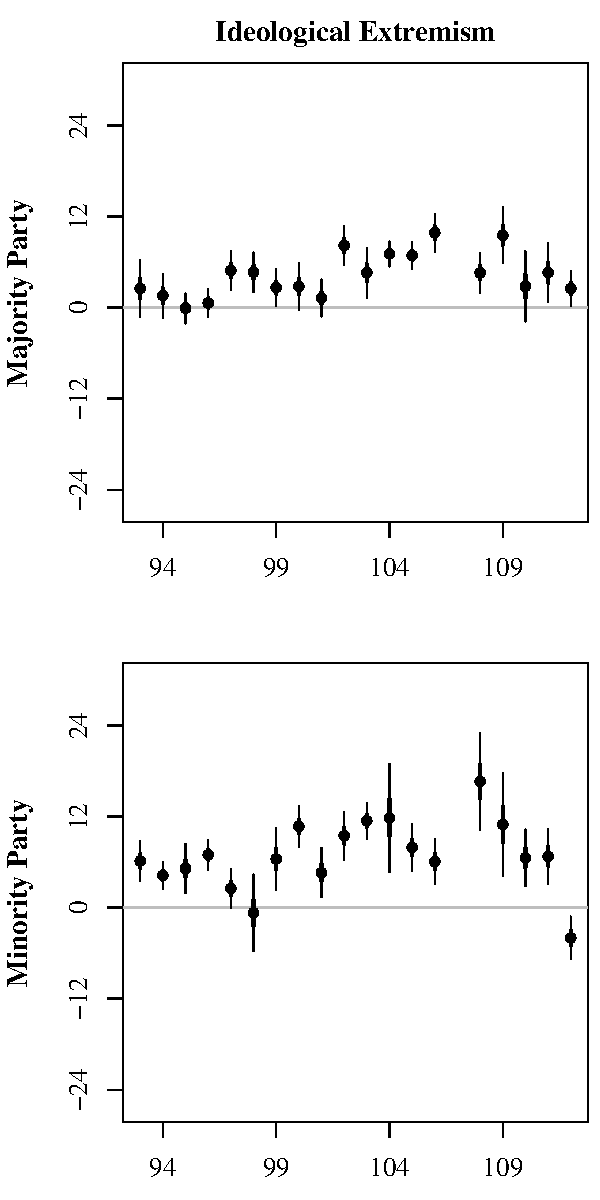
\includegraphics[width = 7cm]{C:/Users/Ethan/Documents/GitHub/partycalls/plots/senate-figure2-lm.pdf}
	\fnote{This coefficient plot is produced by the same formula shown in the Senate regression table with results decomposed by individual Congresses for the Majority and Minority parties. Coefficients shown are for the effect of ideological extremism on party free votes in relation to party call votes. 50\% and 95\% confidence intervals are shown from the points.}
\end{figure}

We note that though ideological extremism is a significant predictor in the regression analyses which rely on all Congresses, it fails to achieve significance for all Congresses taken separately, in the Senate, particularly. We are unsurprised by this since each party in a given Senate has far fewer members than does a party in the House (a few dozen rather than a few hundred). So, we remain largely confident that party calls are present in both chambers and behave in broadly similar ways. 

Having established this, we turn to the case of reelection in the Senate. Initial results point toward different response rates to party calls, but we must also consider whether this difference is across vote types or if it presents itself when analyses focused in changes within Senators, rather than at the aggregate level. We do this in order to show that party calls are a meaningful and useful tool in considering member behavior.

\subsection{Reelection in the Senate}

In this section, we consider the role of proximity to reelection in changing member behavior on different types of votes, separating them into party calls and party free votes. We theorize that member up for reelection will have the preferences of their constituents induced as they approach reelection, one of which is simply that they are different from the party. For this reason, we expect members will be more likely to ignore the call of the party during periods which they are nearing reelection.

To test this, we estimate models which rely on same-state Senator pairs when one of them is up for reelection at the end of the Congress. These pairings are ideal since an expectation is that members will respond according to their voters and same-state Senators are elected by the same voters. So, we are confident in assuming that these pairs will change their behavior in comparable ways as reelection approaches. 

The fact that same-state Senators are not up for reelection at the same time allows us to estimate a generalization of a difference-in-differences design on pairs in Congresses which one is up for reelection. We use this to compare member responsiveness to the party on party calls, the baseline rate of voting with the party, and the difference between these two quantities between the member up for reelection and the member in the beginning or middle of their term. For each of these, a placebo test with randomly assigned treatment is also shown.\footnote{Reported 50\% and 95\% confidence intervals are developed by a bootstrap sample. More details about this and other areas of the methodology can be found in an appendix.} Cases which have more than two Senators from a state during a single Congress (due to deaths and retirements) are dropped from the analysis.

\begin{figure}[H]
	\centering
	\caption{Senate Rate of Voting With Party by Vote Type}
	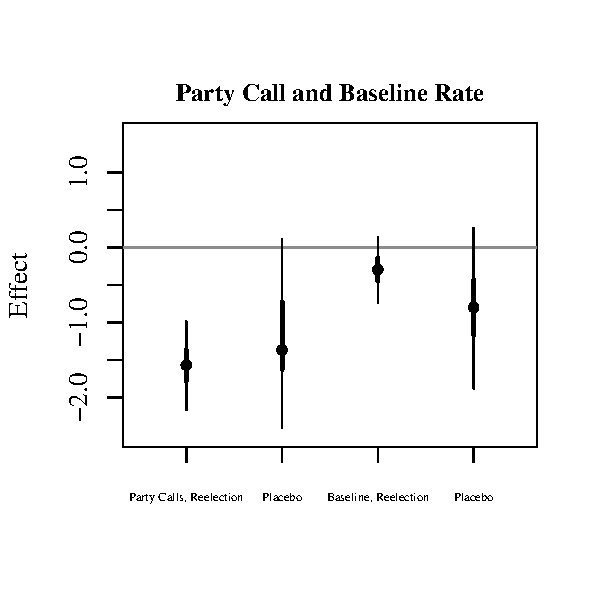
\includegraphics[width = 10cm]{C:/Users/Ethan/Documents/GitHub/partycalls/plots/senate-diff-in-diff-coeff-separate.pdf}
	\fnote{\textit{Note}: This coefficient plot is produced by a paired differences model which uses same-state Senators as a natural pairing. Differences between member responsiveness to party calls are shown by the first two points with the second set representing differences in baseline rate of voting with the party. The first and third columns use proximity to reelection as a treatment which are compared in columns 2 and 4 with a placebo treatment of the Senator with higher seniority in Congresses which neither are up for reelection as a comparison. 50\% and 95\% confidence intervals are shown.}
\end{figure}

\begin{figure}[H]
	\centering
	\caption{Senate Rate of Voting With Party by Vote Type}
	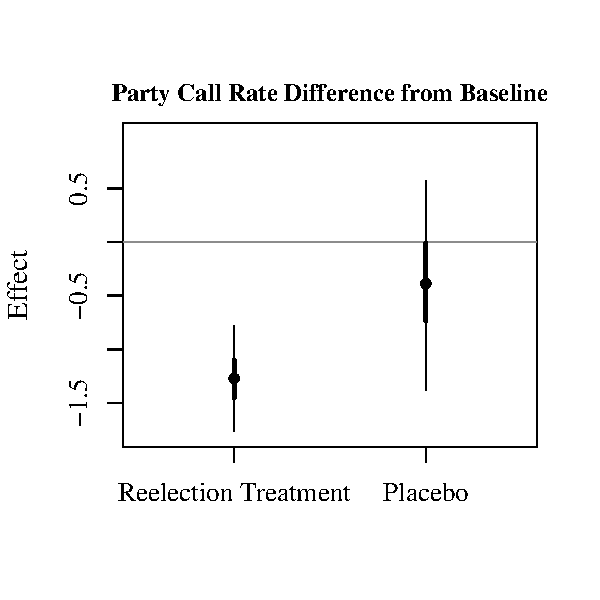
\includegraphics[width = 10cm]{C:/Users/Ethan/Documents/GitHub/partycalls/plots/senate-diff-in-diff-coeff.pdf}
	\fnote{\textit{Note}: This coefficient plot is produced by a paired difference-in-differences model which considers the difference between same-state Senator responsiveness to party calls from their baseline rate of voting with the party. The first column uses proximity to reelection as a treatment while the second uses higher seniority in Congresses which neither is up for reelection as a placebo treatment. 50\% and 95\% confidence intervals are shown.}
\end{figure}

The results of these tests clearly show that member responsiveness to party calls declines, on average, about 1.5\% when they are up for reelection. However, their baseline rate of voting with the party is in line with what would be expected during other Congresses. During the period of analysis, 52\% of votes are classified as party calls and the average rate of responsiveness to party calls is 85\%. The average rate of voting with the party on non-party call votes is 82\%. Thus, while there is still an effect of the call of the party during a period of reelection, the induced preferences of the constituents reduces its impact.

Member voting behavior on other votes does not exhibit this relationship, likely due to them being driven primarily by ideology. Thus, we conclude that party calls are effective at establishing the role of party and ideology in votes.

\subsection{Conclusion}

In this paper, we tested if members respond to party calls in the Senate as they do in the House, using analyses based on those of Minozzi \& Volden (2013). This allowed us not only to confirm their results, but also to show the potential advantages of party calls as a method for viewing member behavior related to ideology and partisanship. We showed that reelection modifies member behavior on roll call votes which party is a factor in, but not those which are based primarily on ideology. 

This is in line with expectations of members working to consider voter preferences more highly as reelection becomes more proximate, though it expands on previous studies by highlighting the votes on which member behavior changes. We determine that party calls are an effective measure for the role of the party in roll call voting behavior and see that conditions shown to affect member's responsiveness to the party affect them but not other vote types.

Having shown this, we believe future work would do well to consider the separation of roll call votes by party calls and non party calls. Doing such could aid immensely in defining the role of party and ideology in member decisions. For instance, the role of increased partisanship viewed through the lens of increases in party calls could prove a worthwhile endeavor.

\pagebreak

\section{Appendices}

\subsection{Appendix A: Detailing the New Sorting Algorithm}

As was done by Minozzi \& Volden (2013) we develop an algorithm to sort votes based on the degree to whether vote choice can be significantly predicted by party or caucus membership after ideology is accounted for. In this algorithm, member ideology in one iteration is calculated on the votes which were not party calls in the previous iteration since party is accounting for some of the weight in decision on the other set. Ideology for the first iteration is calculated on votes which have more than 65\% or less than 35\% of members of the chamber voting on the same side. The algorithm has a 15 iteration burn in period for each Congress. Once this has concluded, the algorithm continues either until the number of votes switched has hit a minimum and begun to climb or until there are fewer than 5 votes which switch between iterations. Once these conditions are met, it continues for 15 additional iterations, the last 5 of which are used to identify party calls and non calls. Any votes which switched between party calls and non party calls during the final 5 iterations are dropped from our analyses.

One of the key changes was the use of the \verb|binIRT()| R function from the \verb|emIRT|in order to calculate members' party free ideology, replacing \verb|ideal()| which was used by Minozzi \& Volden. The \verb|binIRT()| function was developed by Imai, Lo \& Olmsted in order to produce estimates analagous to those of \verb|ideal()| with reduced computational taxation. We find both of these aims to be met.

We find that the party call is not merely produced by a tradeoff of party and ideology explaining different votes; they are on the same side approximately two-thirds of the time in the House and three-fifths of the time in the Senate.

% latex table generated in R 3.3.2 by xtable 1.8-2 package
% Thu Feb 23 17:39:42 2017
\begin{table}[H]
	\centering
	\singlespacing
	\caption{House Sorting Algorithm Coefficient Signs}
	\begin{tabular}{rrr}
		\hline
		& ($-$) Ideal & (+) Ideal \\ 
		\hline
		(-) Party & 0.38 & 0.15 \\ 
		(+) Party & 0.17 & 0.30 \\ 
		\hline
	\end{tabular}
\fnote{The party variable used in this analysis is an indicator for status as a Republican, and thus would be expected to correlate positively with ideal points.}
\end{table}

% latex table generated in R 3.3.2 by xtable 1.8-2 package
% Thu Feb 23 17:23:31 2017
\begin{table}[H]
	\centering
	\singlespacing
	\caption{Senate Sorting Algorithm Coefficient Signs}
	\begin{tabular}{rrr}
		\hline
		& ($-$) Ideal & (+) Ideal \\ 
		\hline
		($-$) Party & 0.33 & 0.16 \\ 
		(+) Party & 0.23 & 0.28 \\ 
		\hline
	\end{tabular}
\fnote{The party variable used in this analysis is an indicator for status as a Republican, and thus would be expected to correlate positively with ideal points.}
\end{table}

We found that the lowered number of both members and bills in the Senate required a few changes to the vote sorting method, however. Since $p$-values will necessarily be lower with fewer observations, we had to change the threshold for party calls to $p <$ 0.05 (from $p <$ 0.01). Next, since the ideal point algorithm uses a logistic regression, problems arose in vote sorting when we also tried to use another to sort vote type with this in the Senate. Neither change leads the sorting in the House to differ for the most part. We find that the sorting of close and lopsided votes by this method to be in line with Minozzi \& Volden's findings.

% latex table generated in R 3.3.2 by xtable 1.8-2 package
% Mon Mar 20 13:02:44 2017
\begin{table}[H]
	\centering
	\singlespacing
	\caption{House Vote Coding for Close and Lopsided Votes} 
	\begin{tabular}{lrr}
		\hline
		& Party Call & Noncall \\ 
		\hline
		Lopsided & 4245 & 6123 \\ 
		Close & 9308 & 1090 \\ 
		\hline
	\end{tabular}
\fnote{The threshold for a vote to be lopsided was 65\% of members (or conversely, 35\%) voting on the same side of a roll call vote.}
\end{table}

% latex table generated in R 3.3.2 by xtable 1.8-2 package
% Mon Mar 20 13:04:18 2017
\begin{table}[H]
	\centering
	\singlespacing
	\caption{Senate Vote Coding for Close and Lopsided Votes} 
	\begin{tabular}{lrr}
		\hline
		& Party Call & Noncall \\ 
		\hline
		Lopsided & 2063 & 4876 \\ 
		Close & 5233 & 1851 \\ 
		\hline
	\end{tabular}
\fnote{The threshold for a vote to be lopsided was 65\% of members (or conversely, 35\%) voting on the same side of a roll call vote.}
\end{table}













\subsection{Appendix B: Methodology for Senate Reelection Section}

In order to better test the role of reelection we use same-state senators as a natural pairing. These results were shown in figures 2 and 3 in the paper. The analyses we performed on these pairs were generalizations of the difference in differences design, in which the member not up for reelection had their response rate subtracted from that of the member who was up for reelection. Figure 2 showed the differences by vote type and figure 3 showed the change between vote types between these pairs. For each of these, we also performed analyses on Congresses which neither was up for reelection as a placebo test, with the ``treatment'' being based on which member was more senior. Here we show the results in tables, with breakdowns by seat pair type.

% latex table generated in R 3.3.2 by xtable 1.8-2 package
% Mon Mar 27 22:28:47 2017
\begin{table}[H]
	\centering
	\singlespacing
	\caption{Reelection and Response to Party Calls, Difference in Differences} 
	\begin{tabular}{llrrr}
		\hline
		Test & DV & Estimate & Lower Bound & Upper Bound \\ 
		\hline
		Effect & pirate100 & -1.569 & -2.139 & -1.001 \\ 
		Placebo & pirate100 & -0.331 & -1.281 & 1.259 \\ 
		Effect & pfrate100 & -0.297 & -0.798 & 0.126 \\ 
		Placebo & pfrate100 & -0.644 & -1.074 & 1.143 \\ 
		\hline
	\end{tabular}
\end{table}

% latex table generated in R 3.3.2 by xtable 1.8-2 package
% Mon Mar 27 22:28:47 2017
\begin{table}[H]
	\centering
	\singlespacing
	\caption{Diff in Diff, Subgroup Condition, Party Influenced Rate} 
	\begin{tabular}{llr}
		\hline
		Test & DV & Estimate \\ 
		\hline
		2 Maj Dems Effect & pirate100 & 0.0708958 \\ 
		2 Maj Dems Placebo & pirate100 & -0.4769119 \\ 
		2 Min Dems Effect & pirate100 & -1.8733904 \\ 
		2 Min Dems Placebo & pirate100 & -1.2633351 \\ 
		2 Maj Reps Effect & pirate100 & -1.1307379 \\ 
		2 Maj Reps Placebo & pirate100 & -2.2707921 \\ 
		2 Min Reps Effect & pirate100 & 0.3990873 \\ 
		2 Min Reps Placebo & pirate100 & -1.9947329 \\ 
		Split, Maj Dem, Dem Effect & pirate100 & 3.8789004 \\ 
		Split, Maj Dem, Dem Placebo & pirate100 & 0.7159106 \\ 
		Split, Maj Dem, Rep Effect & pirate100 & -8.6767819 \\ 
		Split, Maj Dem, Rep Placebo & pirate100 & -1.0729345 \\ 
		Split, Maj Rep, Dem Effect & pirate100 & -8.0169523 \\ 
		Split, Maj Rep, Dem Placebo & pirate100 & -2.1276690 \\ 
		Split, Maj Rep, Rep Effect & pirate100 & 0.0096892 \\ 
		Split, Maj Rep, Rep Placebo & pirate100 & 0.0232939 \\ 
		\hline
	\end{tabular}
\end{table}

% latex table generated in R 3.3.2 by xtable 1.8-2 package
% Sun Mar 26 19:10:24 2017
\begin{table}[H]
	\centering
	\singlespacing
	\caption{Reelection and Response to Party Calls, Difference in Differences} 
	\begin{tabular}{llrrr}
		\hline
		test & DV & Estimate & Lower Bound & Upper Bound \\ 
		\hline
		Effect & pirate100 - pfrate100 & -1.272 & -1.775 & -0.794 \\ 
		Placebo & pirate100 - pfrate100 & -0.292 & -0.904 & 0.935 \\ 
		\hline
	\end{tabular}
\end{table}

% latex table generated in R 3.3.2 by xtable 1.8-2 package
% Sun Mar 26 19:10:27 2017
\begin{table}[H]
	\centering
	\caption{Diff in Diff, Subgroup Condition, Party Influenced Rate} 
	\begin{tabular}{llr}
		\hline
		Test & DV & Estimate \\ 
		\hline
		2 Maj Dems Effect & pirate100 - pfrate100 & -0.1191943 \\ 
		2 Maj Dems Placebo & pirate100 - pfrate100 & 0.5657017 \\ 
		2 Min Dems Effect & pirate100 - pfrate100 & -1.8253378 \\ 
		2 Min Dems Placebo & pirate100 - pfrate100 & -0.4463733 \\ 
		2 Maj Reps Effect & pirate100 - pfrate100 & -2.2112471 \\ 
		2 Maj Reps Placebo & pirate100 - pfrate100 & -0.1749949 \\ 
		2 Min Reps Effect & pirate100 - pfrate100 & 0.7774782 \\ 
		2 Min Reps Placebo & pirate100 - pfrate100 & -0.4516436 \\ 
		Split, Maj Dem, Dem Effect & pirate100 - pfrate100 & -0.8756821 \\ 
		Split, Maj Dem, Dem Placebo & pirate100 - pfrate100 & -1.8454871 \\ 
		Split, Maj Dem, Rep Effect & pirate100 - pfrate100 & -1.4582552 \\ 
		Split, Maj Dem, Rep Placebo & pirate100 - pfrate100 & 0.0117995 \\ 
		Split, Maj Rep, Dem Effect & pirate100 - pfrate100 & -7.1166813 \\ 
		Split, Maj Rep, Dem Placebo & pirate100 - pfrate100 & -3.4630959 \\ 
		Split, Maj Rep, Rep Effect & pirate100 - pfrate100 & 0.3772151 \\ 
		Split, Maj Rep, Rep Placebo & pirate100 - pfrate100 & 0.2964502 \\ 
		\hline
	\end{tabular}
\end{table}

As a further test, not shown in the paper, we estimated the effect of reelection and other variables with a fixed effects model. This produces substantively similar effects to those reported in the main paper. Most notable to us is that the effect produced by being up for reelection is in line with findings shown in the main paper.

\begin{table}[H]
	\begin{center}
		\caption{Senate Fixed Effects Models, Party Call Response Rate}
		\begin{tabular}{l c c c c }
			\hline
			& Democrats & Republicans & Majority & Minority \\
			\hline
			Ideological Extremism  & $2.88^{***}$ & $4.00^{***}$  & $1.80^{**}$   & $3.93^{***}$ \\
			& $(0.69)$     & $(0.75)$      & $(0.64)$      & $(0.97)$     \\
			Baseline Rate of Voting with Party               & $0.37^{***}$ & $0.25^{***}$  & $0.37^{***}$  & $0.18^{*}$   \\
			& $(0.05)$     & $(0.05)$      & $(0.05)$      & $(0.07)$     \\
			Up For Reelection     & $-0.55^{*}$  & $-1.55^{***}$ & $-1.02^{***}$ & $-1.04^{**}$ \\
			& $(0.27)$     & $(0.34)$      & $(0.28)$      & $(0.37)$     \\
			Vote Share             & $0.03$       & $-0.05$       & $0.02$        & $-0.02$      \\
			& $(0.02)$     & $(0.03)$      & $(0.03)$      & $(0.04)$     \\
			Presidential Vote Share       & $0.27^{***}$ & $0.09$        & $0.31^{***}$  & $0.14^{*}$   \\
			& $(0.04)$     & $(0.05)$      & $(0.06)$      & $(0.06)$     \\
			Freshman                & $0.71$       & $0.98^{*}$    & $0.77$        & $0.78$       \\
			& $(0.48)$     & $(0.46)$      & $(0.46)$      & $(0.76)$     \\
			Retiree                 & $0.25$       & $0.88$        & $0.36$        & $0.75$       \\
			& $(0.83)$     & $(0.83)$      & $(0.99)$      & $(0.91)$     \\
			Best Committee         & $0.14$       & $0.11$        & $0.29$        & $0.36^{*}$   \\
			& $(0.12)$     & $(0.16)$      & $(0.15)$      & $(0.18)$     \\
			Power Committee        & $-0.48$      & $-0.22$       & $-1.26$       & $-0.45$      \\
			& $(0.70)$     & $(0.98)$      & $(0.89)$      & $(1.01)$     \\
			Leader                  & $0.87$       & $1.46^{*}$    & $1.39$        & $1.31$       \\
			& $(0.47)$     & $(0.62)$      & $(0.78)$      & $(0.80)$     \\
			Committee Chair                   & $0.38$       & $0.65$        & $-0.57$       &              \\
			& $(0.64)$     & $(0.71)$      & $(0.56)$      &              \\
			\hline
			Num. obs.               & 1042         & 951           & 1052          & 843          \\
			R$^2$      & 0.89         & 0.91          & 0.92          & 0.94         \\
			Adj. R$^2$ & 0.87         & 0.88          & 0.89          & 0.91         \\
			\hline
			\multicolumn{5}{l}{\scriptsize{$^{***}p<0.001$, $^{**}p<0.01$, $^*p<0.05$}}
		\end{tabular}
	\end{center}
\end{table}

\subsection{Appendix C: Other Tables and Figures from Replication}

In Minozzi \& Volden (2013), the regression table produced shows results in Congresses 97, 102, and 107 divided by party. Here, we produce the results from our analyses in the House of these chambers for ideological extremism\footnote{Since distance from floor median was not calculated for or used by any of our analyses, we do not replicate any of their analyses which use it}.

\begin{table}
	\begin{center}
		\caption{Replication of Minozzi \& Volden (2013), Table 3}
		\begin{tabular}{l c c c c c c }
			\hline
			& \multicolumn{3}{c}{Democrats} & \multicolumn{3}{c}{Republicans} \\
			\cline{2-7}
			& 97th & 102nd & 107th & 97th & 102nd & 107th \\
			\hline
			Ideological Extremism & $9.34^{***}$   & $4.76^{***}$ & $-1.03$       & $5.15^{***}$ & $6.48^{***}$  & $-0.29$       \\
			& $(0.53)$       & $(0.68)$     & $(1.42)$      & $(0.71)$     & $(0.76)$      & $(0.61)$      \\
			Baseline Rate of Voting With Party              & $1.04^{***}$   & $0.69^{***}$ & $1.06^{**}$   & $0.51^{***}$ & $0.44^{***}$  & $0.35^{**}$   \\
			& $(0.07)$       & $(0.08)$     & $(0.34)$      & $(0.08)$     & $(0.08)$      & $(0.11)$      \\
			Vote Share            & $-0.10^{*}$    & $-0.13^{**}$ & $-0.28^{***}$ & $0.03$       & $-0.13$       & $-0.09^{*}$   \\
			& $(0.05)$       & $(0.04)$     & $(0.07)$      & $(0.06)$     & $(0.07)$      & $(0.04)$      \\
			Pres. Vote Share      & $0.15^{**}$    & $0.20^{***}$ & $0.36^{***}$  & $0.24^{***}$ & $0.26^{**}$   & $0.20^{***}$  \\
			& $(0.05)$       & $(0.05)$     & $(0.06)$      & $(0.07)$     & $(0.08)$      & $(0.04)$      \\
			Party Leader                 & $6.42^{*}$     & $2.29$       & $0.38$        & $0.50$       & $3.75$        & $3.45^{**}$   \\
			& $(2.90)$       & $(1.92)$     & $(2.30)$      & $(2.42)$     & $(2.22)$      & $(1.22)$      \\
			Committee Chair                  & $2.53$         & $1.21$       &               &              &               & $1.39$        \\
			& $(1.52)$       & $(1.32)$     &               &              &               & $(0.90)$      \\
			Power Committee                 & $1.03$         & $1.34$       & $-1.08$       & $-1.19$      & $0.34$        & $-0.27$       \\
			& $(1.02)$       & $(0.89)$     & $(1.26)$      & $(1.34)$     & $(1.40)$      & $(0.63)$      \\
			Best Committee          & $0.08$         & $-0.06$      & $0.23^{*}$    & $0.10$       & $0.09$        & $0.17^{**}$   \\
			& $(0.08)$       & $(0.08)$     & $(0.09)$      & $(0.09)$     & $(0.11)$      & $(0.05)$      \\
			Female                 & $0.12$         & $-1.42$      & $2.03$        & $-4.12^{*}$  & $-1.66$       & $-1.41$       \\
			& $(2.07)$       & $(1.20)$     & $(1.14)$      & $(2.01)$     & $(2.22)$      & $(0.83)$      \\
			African American                   & $-2.38$        & $-1.90$      & $-1.53$       &              & $3.22$        & $-3.62$       \\
			& $(2.13)$       & $(1.55)$     & $(1.66)$      &              & $(6.08)$      & $(3.55)$      \\
			Latino                 & $3.83$         & $2.51$       & $1.24$        & $-1.65$      & $2.48$        & $0.69$        \\
			& $(2.93)$       & $(1.86)$     & $(1.81)$      & $(5.79)$     & $(6.27)$      & $(1.48)$      \\
			South                  & $-4.73^{***}$  & $-1.23$      & $-3.09^{*}$   & $1.91$       & $0.06$        & $1.47^{**}$   \\
			& $(1.02)$       & $(0.77)$     & $(1.19)$      & $(1.15)$     & $(1.16)$      & $(0.51)$      \\
			Seniority              & $0.11$         & $0.08$       & $-0.00$       & $-0.02$      & $-0.71^{***}$ & $-0.16^{*}$   \\
			& $(0.12)$       & $(0.10)$     & $(0.13)$      & $(0.17)$     & $(0.15)$      & $(0.08)$      \\
			Freshman               & $-0.93$        & $-0.29$      & $-0.97$       & $3.06^{*}$   & $2.87$        & $0.37$        \\
			& $(1.42)$       & $(1.16)$     & $(1.90)$      & $(1.35)$     & $(1.78)$      & $(0.78)$      \\
			Intercept            & $-23.98^{***}$ & $18.85^{*}$  & $-39.78$      & $13.21$      & $23.66^{**}$  & $44.77^{***}$ \\
			& $(6.79)$       & $(7.28)$     & $(33.81)$     & $(8.22)$     & $(7.78)$      & $(10.25)$     \\
			\hline
			R$^2$                  & 0.81           & 0.67         & 0.41          & 0.53         & 0.62          & 0.53          \\
			Adj. R$^2$             & 0.80           & 0.65         & 0.37          & 0.50         & 0.59          & 0.50          \\
			Num. obs.              & 233            & 263          & 209           & 187          & 162           & 217           \\
			RMSE                   & 5.49           & 4.88         & 6.12          & 5.63         & 5.79          & 3.24          \\
			\hline
			\multicolumn{7}{l}{\scriptsize{$^{***}p<0.001$, $^{**}p<0.01$, $^*p<0.05$}}
		\end{tabular}
	\end{center}
\end{table}























































\end{document}